\documentclass[12pt]{article}
\textwidth 16.5cm
\textheight 23.5cm
\oddsidemargin 0pt
\topmargin -2cm
% \usepackage{epsf}

% Writing maths
\usepackage{
    amsmath, % aligns, equations, etc.
    amsfonts, % blackboard bold, etc.
    bbm, % blackboard bold for numbers.
}

% Figures
\usepackage{graphicx}

% References
\usepackage{hyperref}

% References 
\usepackage{natbib}
\bibliographystyle{natbib}
\setcitestyle{authoryear, open={(},close={)}}

% Inline comments from Jacob and Bella
\usepackage{xcolor}
\usepackage[draft,inline,nomargin,index]{fixme}
\fxsetup{theme=color,mode=multiuser}
\FXRegisterAuthor{jb}{ajb}{\color{blue} JB}
\FXRegisterAuthor{bd}{abd}{\color{red} BD}

\title{Simulations of Immigration Queues at Edinburgh Airport: Tech Setup}
 \author{Jacob R. Bradley
 \\ \emph{School of Mathematics, University of Edinburgh}}

\begin{document}
\maketitle

\section{Introduction}
This document contains descriptions of how GitHub, RStudio, Overleaf, and Zotero interact for a (hopefully) seamless and ultra-efficient competition-smashing workflow!

\section{Methods}
\subsection{GitHub}
The code for this project is held in a \href{https://github.com/cobrbra/immigration_queue_simulation_edinburgh_airport}{GitHub repository}. This stores and tracks the history of all the data, code, and docs associated with the project, but shouldn't be used directly for editing anything aside from in an emergency! Instead, coding should be done in RStudio and writing should be done in Overleaf. In GitHub, you can see the entire project folder layout (Figure~\ref{fig:github_overview}).

\begin{figure}[htbp]
    \centering
    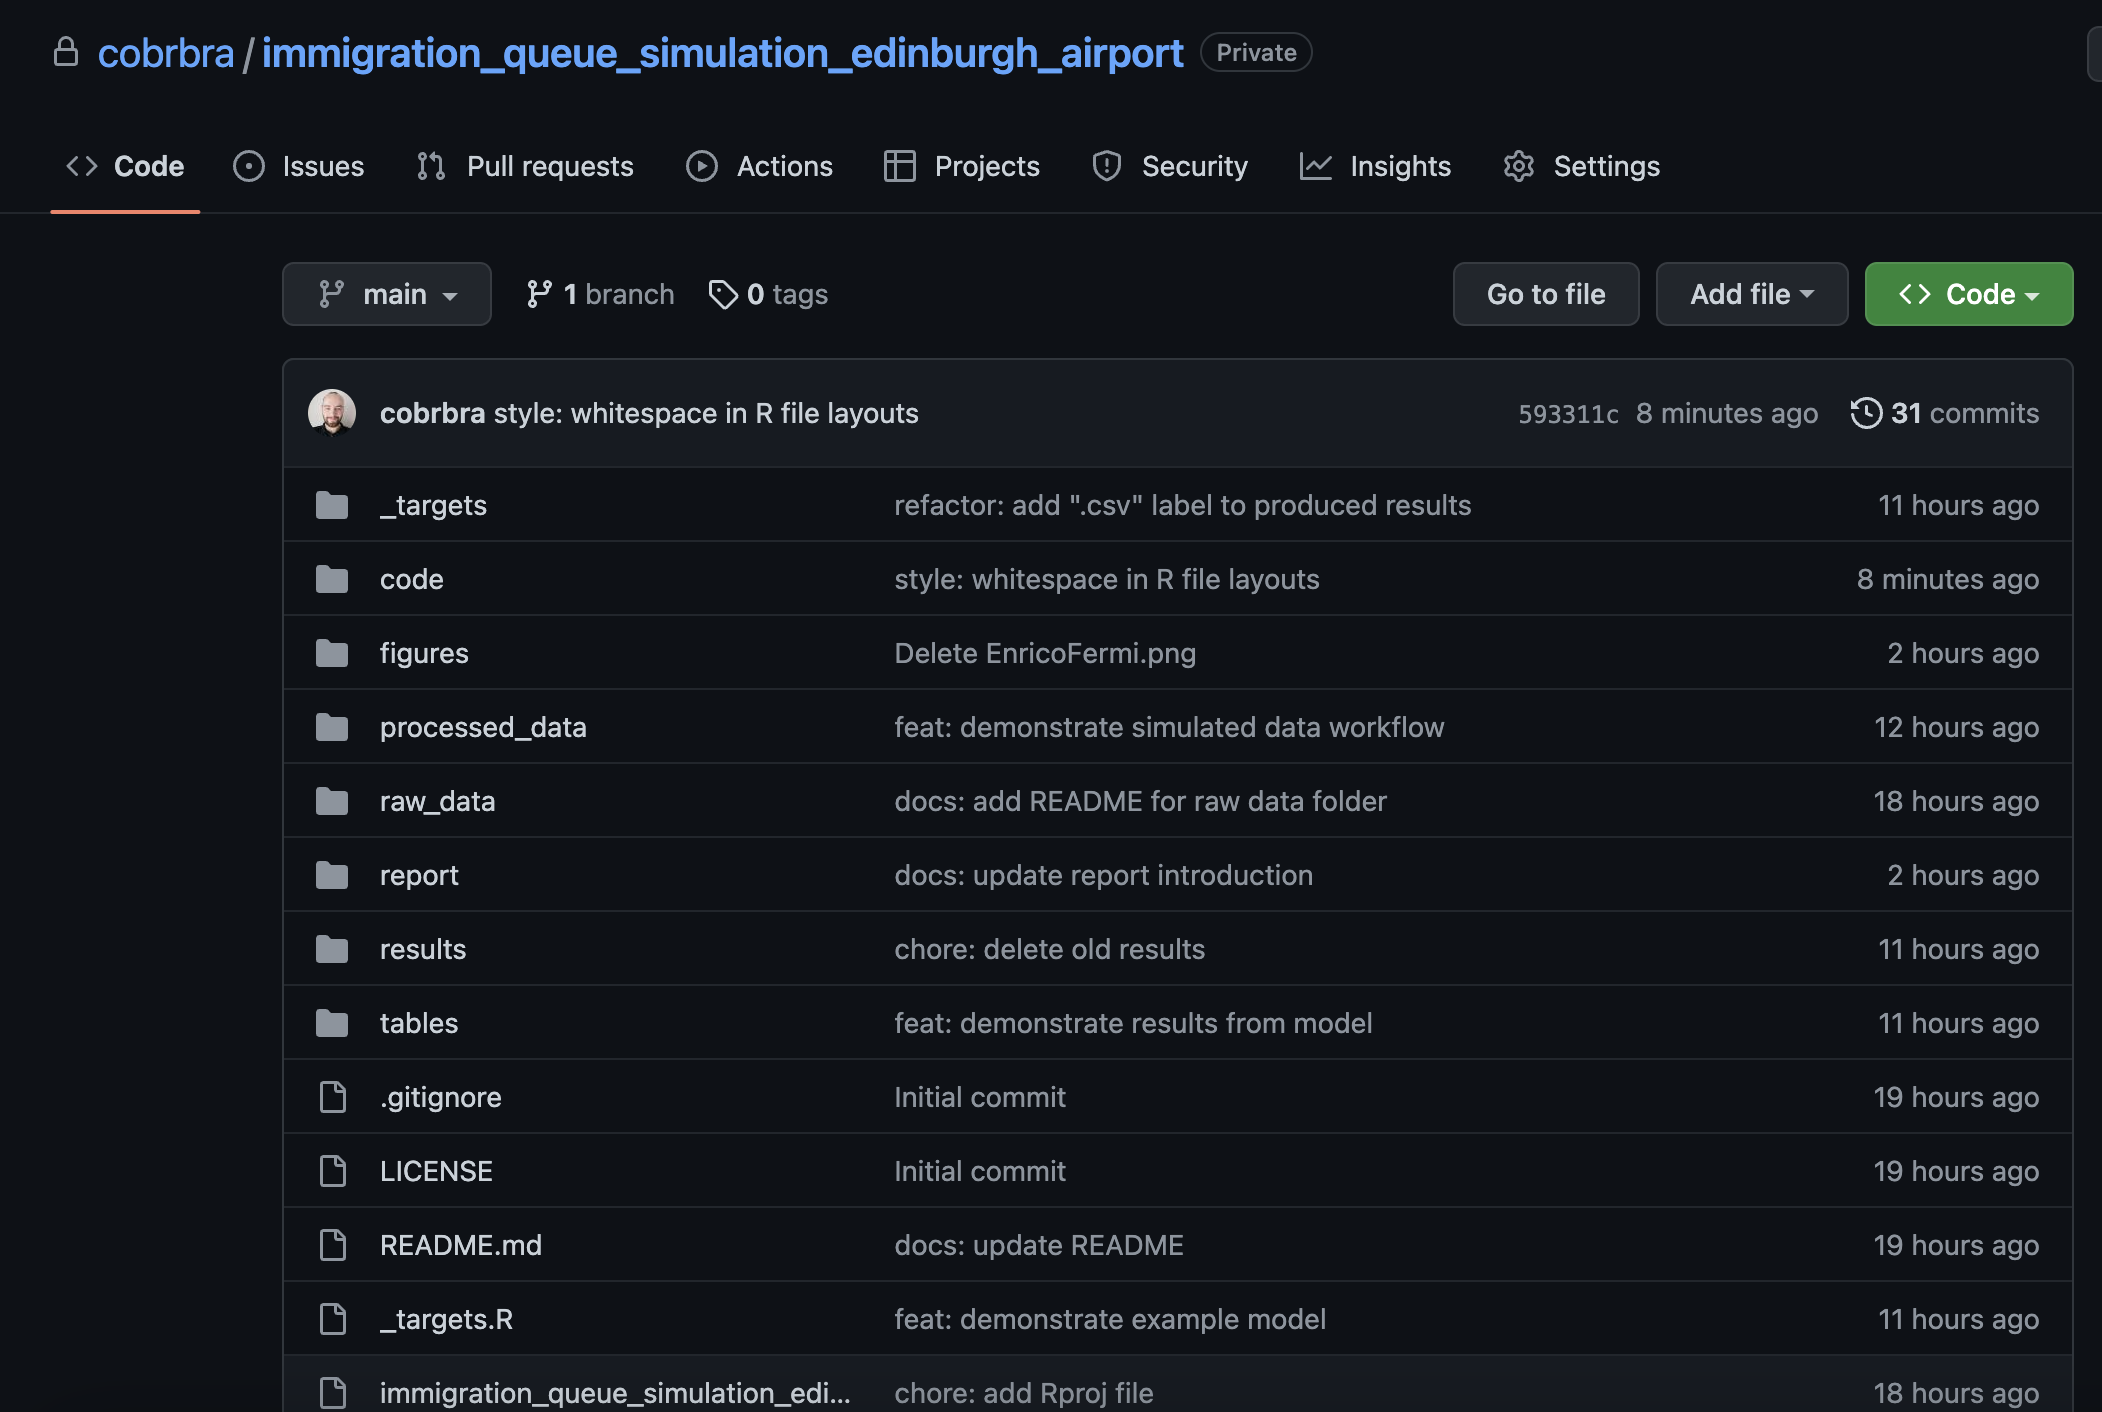
\includegraphics[width=4in]{figures/github_overview.png}
    \caption{GitHub view of project folder.}
    \label{fig:github_overview}
\end{figure}

The ``Code'' tab will be useful for syncing GitHub with RStudio (see below). Syncing with Overleaf should already have been done from here.

\subsection{RStudio}
RStudio will be where (separately) we each do coding for the project. We'll each have our own ``local'' copy, which will be linked to GitHub, where the ``main'' copy will be stored. When we want to share some of the changes we've made, we'll ``commit'' them (i.e. select which changes are ready to be shared) and then ``push'' them. When we want to update with other changes that have been made, we'll ``pull'' these from the main version in GitHub. 

To get started, we'll need to set up the repository as a project in RStudio. You can do this with \texttt{File} $\rightarrow$ \texttt{New Project} $\rightarrow$ \texttt{Version Control} $\rightarrow$ \texttt{Git}. You should then enter the repository URL \href{git@github.com:cobrbra/immigration_queue_simulation_edinburgh_airport.git}{git@github.com:cobrbra/immigration\textunderscore queue\textunderscore simulation\textunderscore edinburgh\textunderscore airport.git} (we'll need to do some faffing around with ssh keys i.e. permissions, but that'll be a one-time thing). You should put the repository name (not including my GitHub handle) as the project name and choose where in your system you want it all stored (see Figure~\ref{fig:rstudio_new_project}. 

\begin{figure}[htbp]
    \centering
    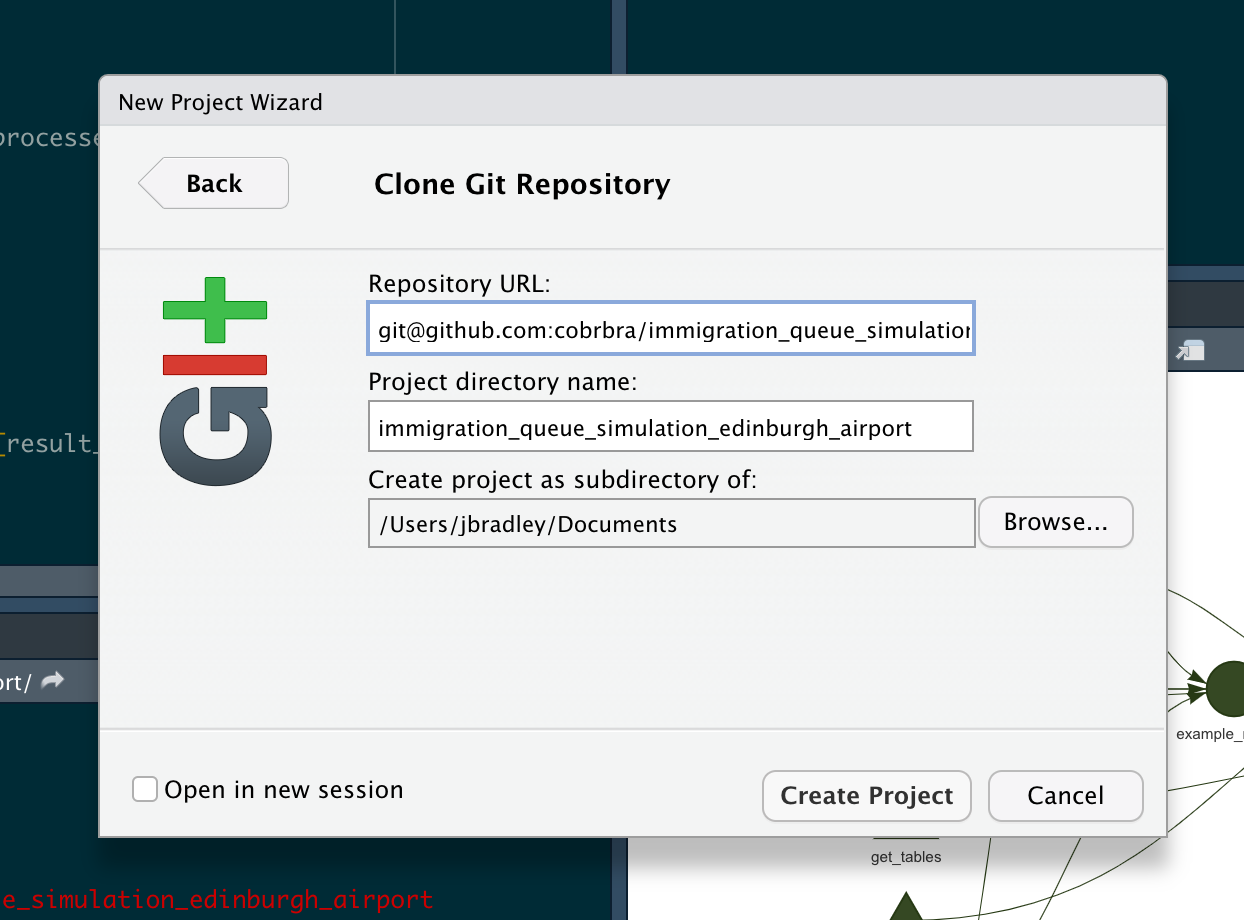
\includegraphics[width=4in]{figures/rstudio_new_project.png}
    \caption{Creating a new project from Git in RStudio.}
    \label{fig:rstudio_new_project}
\end{figure}

\subsection{Overleaf}
\subsection{Zotero}
\subsection{Targets}

% \section{Results}

% \begin{figure}[htbp]
%     \centering
%     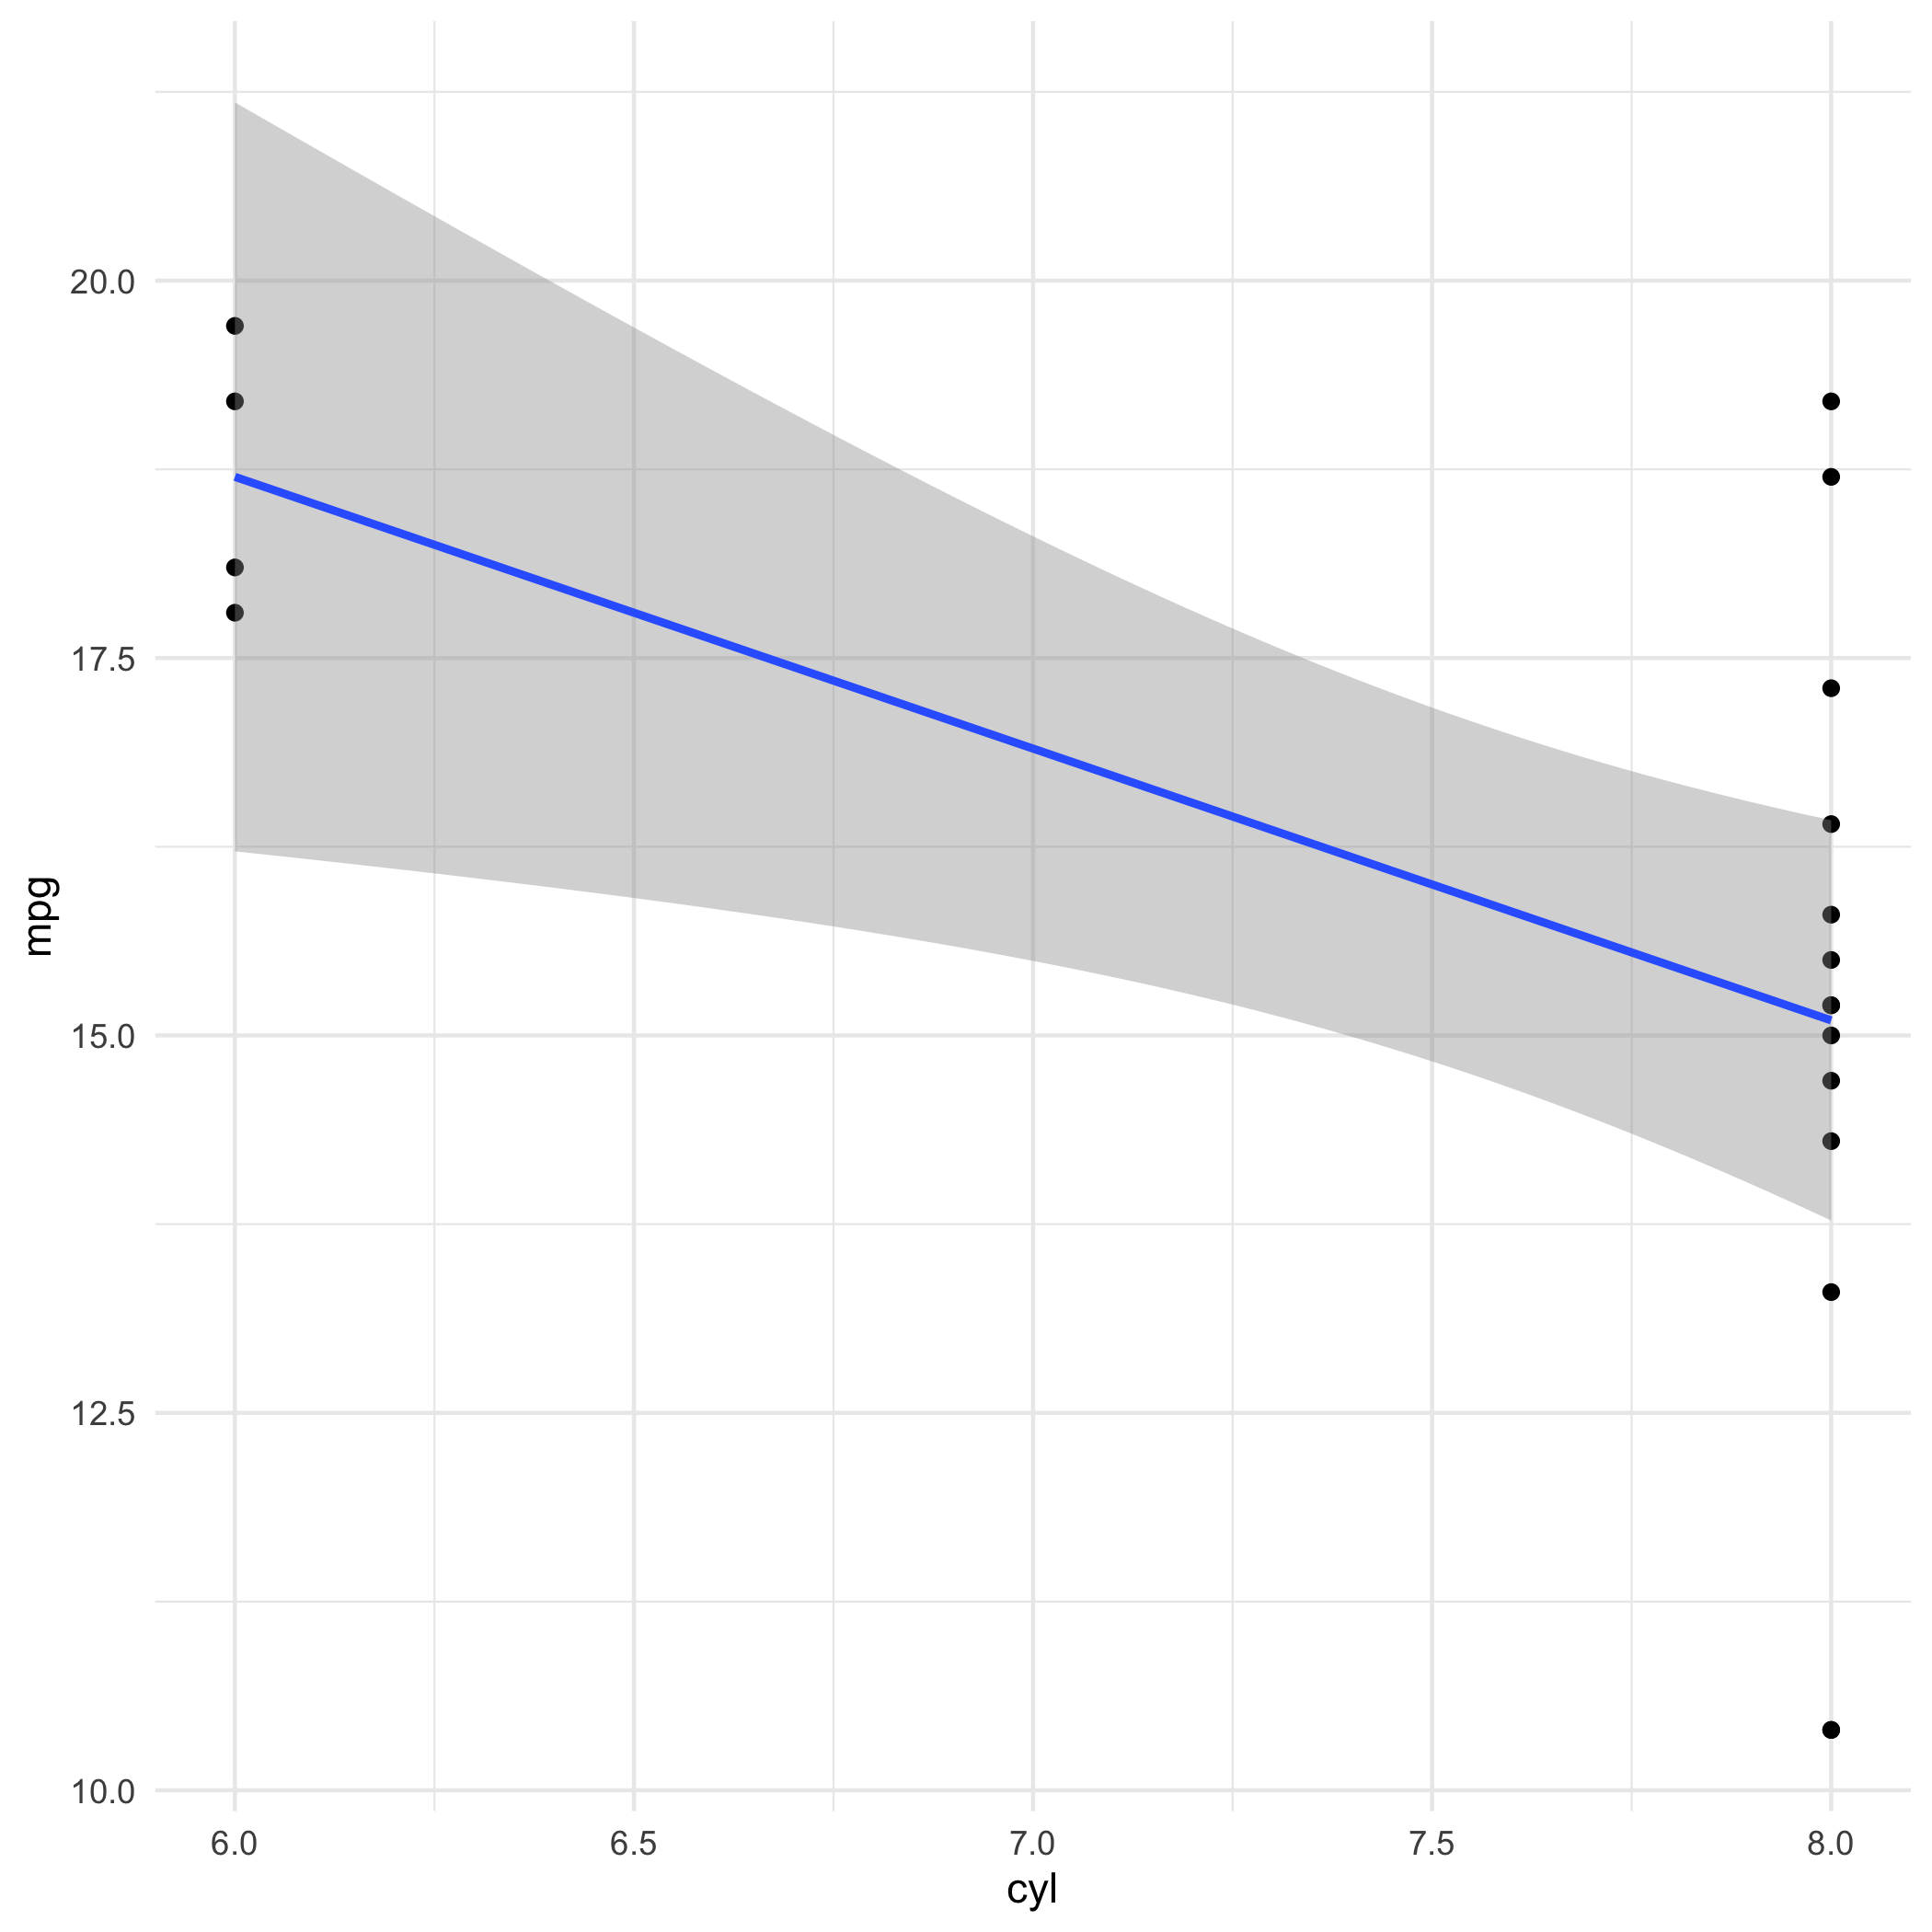
\includegraphics[width=4in]{figures/mt_cars_summary.png}
%     \caption{Example figure generated from mtcars workflow.}
%     \label{fig:mtcars}
% \end{figure}

% \begin{figure}[htbp]
%     \centering
%     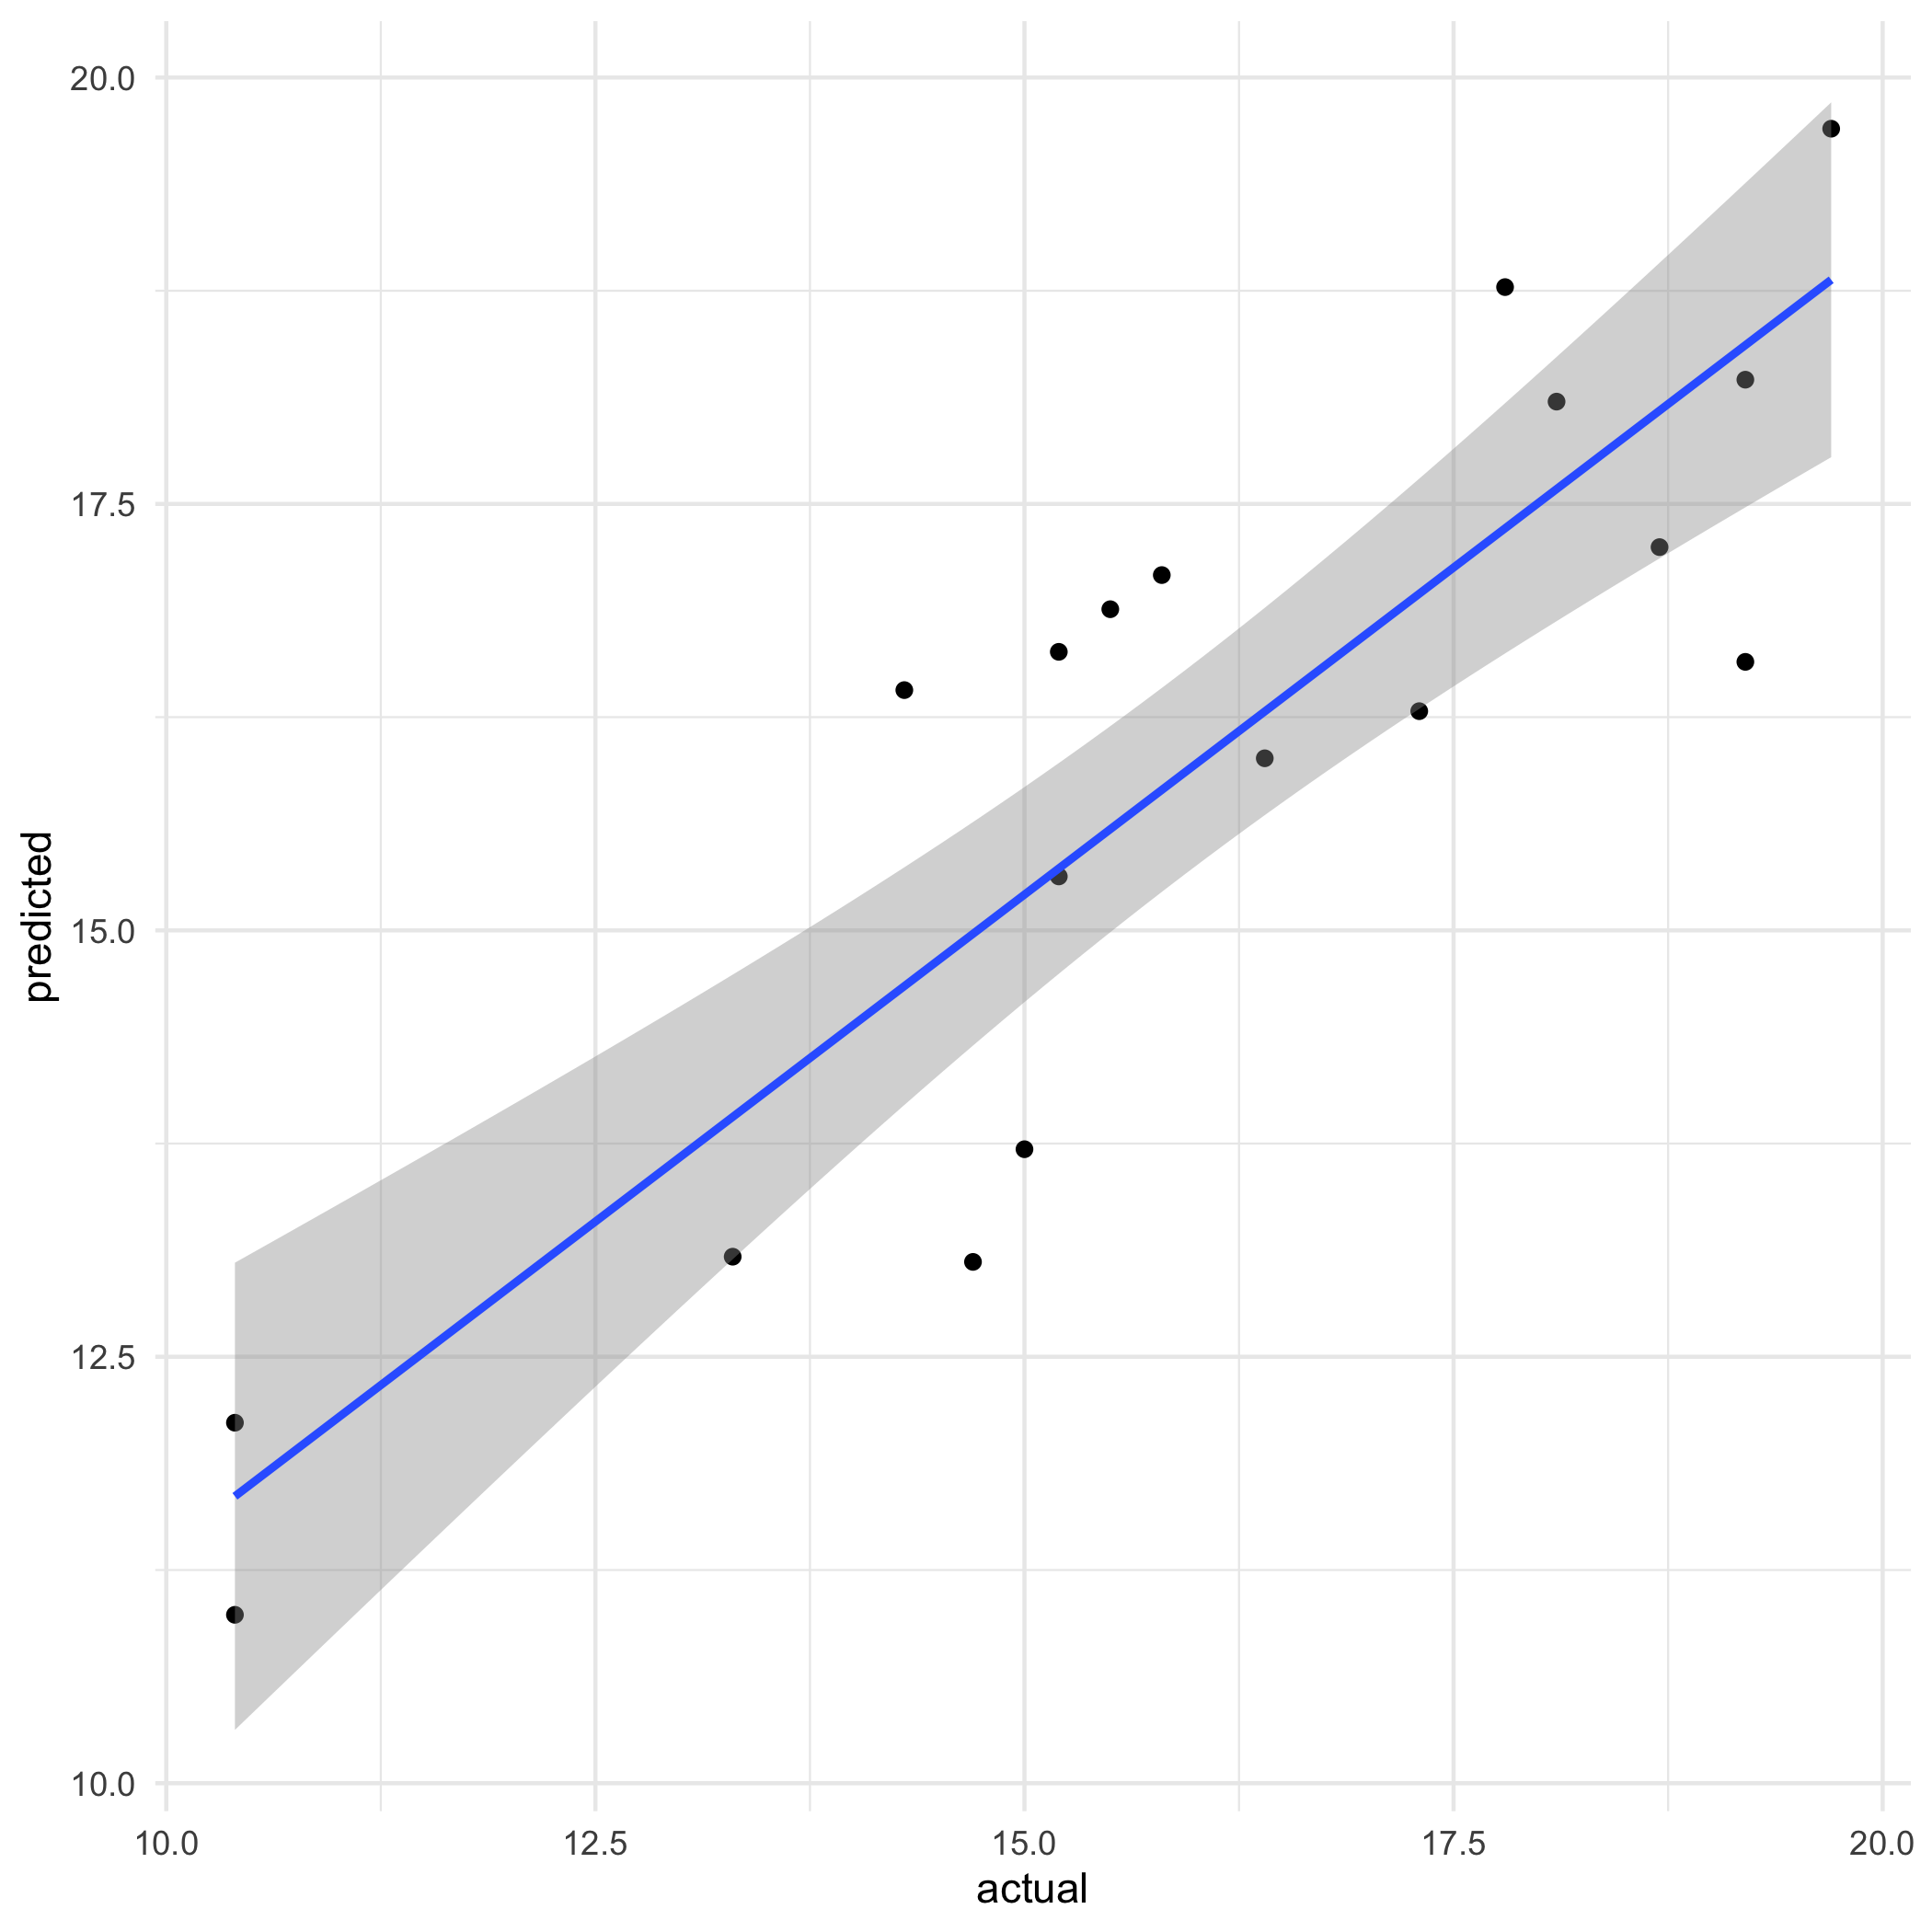
\includegraphics[width=4in]{figures/mpg_model_actual_vs_predicted.png}
%     \caption{Example figure generated from a model of mtcars data.}
%     \label{fig:mtcars_model}
% \end{figure}

% % latex table generated in R 4.2.2 by xtable 1.8-4 package
% Wed Feb 22 17:14:53 2023
\begin{table}[ht]
\centering
\begin{tabular}{rrrrrrrrrrrr}
  \hline
 & mpg & cyl & disp & hp & drat & wt & qsec & vs & am & gear & carb \\ 
  \hline
1 & 18.70 & 8.00 & 360.00 & 175.00 & 3.15 & 3.44 & 17.02 & 0.00 & 0.00 & 3.00 & 2.00 \\ 
  2 & 18.10 & 6.00 & 225.00 & 105.00 & 2.76 & 3.46 & 20.22 & 1.00 & 0.00 & 3.00 & 1.00 \\ 
  3 & 14.30 & 8.00 & 360.00 & 245.00 & 3.21 & 3.57 & 15.84 & 0.00 & 0.00 & 3.00 & 4.00 \\ 
  4 & 19.20 & 6.00 & 167.60 & 123.00 & 3.92 & 3.44 & 18.30 & 1.00 & 0.00 & 4.00 & 4.00 \\ 
  5 & 17.80 & 6.00 & 167.60 & 123.00 & 3.92 & 3.44 & 18.90 & 1.00 & 0.00 & 4.00 & 4.00 \\ 
  6 & 16.40 & 8.00 & 275.80 & 180.00 & 3.07 & 4.07 & 17.40 & 0.00 & 0.00 & 3.00 & 3.00 \\ 
  7 & 17.30 & 8.00 & 275.80 & 180.00 & 3.07 & 3.73 & 17.60 & 0.00 & 0.00 & 3.00 & 3.00 \\ 
  8 & 15.20 & 8.00 & 275.80 & 180.00 & 3.07 & 3.78 & 18.00 & 0.00 & 0.00 & 3.00 & 3.00 \\ 
  9 & 10.40 & 8.00 & 472.00 & 205.00 & 2.93 & 5.25 & 17.98 & 0.00 & 0.00 & 3.00 & 4.00 \\ 
  10 & 10.40 & 8.00 & 460.00 & 215.00 & 3.00 & 5.42 & 17.82 & 0.00 & 0.00 & 3.00 & 4.00 \\ 
  11 & 14.70 & 8.00 & 440.00 & 230.00 & 3.23 & 5.34 & 17.42 & 0.00 & 0.00 & 3.00 & 4.00 \\ 
  12 & 15.50 & 8.00 & 318.00 & 150.00 & 2.76 & 3.52 & 16.87 & 0.00 & 0.00 & 3.00 & 2.00 \\ 
  13 & 15.20 & 8.00 & 304.00 & 150.00 & 3.15 & 3.44 & 17.30 & 0.00 & 0.00 & 3.00 & 2.00 \\ 
  14 & 13.30 & 8.00 & 350.00 & 245.00 & 3.73 & 3.84 & 15.41 & 0.00 & 0.00 & 3.00 & 4.00 \\ 
  15 & 19.20 & 8.00 & 400.00 & 175.00 & 3.08 & 3.85 & 17.05 & 0.00 & 0.00 & 3.00 & 2.00 \\ 
  16 & 15.80 & 8.00 & 351.00 & 264.00 & 4.22 & 3.17 & 14.50 & 0.00 & 1.00 & 5.00 & 4.00 \\ 
  17 & 19.70 & 6.00 & 145.00 & 175.00 & 3.62 & 2.77 & 15.50 & 0.00 & 1.00 & 5.00 & 6.00 \\ 
  18 & 15.00 & 8.00 & 301.00 & 335.00 & 3.54 & 3.57 & 14.60 & 0.00 & 1.00 & 5.00 & 8.00 \\ 
   \hline
\end{tabular}
\caption{MTCars dataset restricted to observations with $<20$ miles per gallon \label{tab:mtcars_full}} 
\end{table}


% \section{Discussion}
% \section{Conclusion}
% \bibliography{references.bib}
\end{document}